\documentclass[]{article}
\usepackage[latin1]{inputenc}
\usepackage{amsmath,amssymb,bm} % math stuff
\usepackage[top=1.85cm, bottom=1.65cm, left=2.2cm, right=2.2cm]{geometry}

% FOR DISPLAYING CODE
\usepackage{listings}
\usepackage{color}
\definecolor{dkgreen}{rgb}{0,0.6,0}
\definecolor{gray}{rgb}{0.5,0.5,0.5}
\definecolor{mauve}{rgb}{0.58,0,0.82}

\lstset{frame=tb,
	language=Python,
	aboveskip=3mm,
	belowskip=3mm,
	showstringspaces=false,
	columns=flexible,
	basicstyle={\small\ttfamily},
	numbers=none,
	numberstyle=\tiny\color{gray},
	keywordstyle=\color{blue},
	commentstyle=\color{dkgreen},
	stringstyle=\color{mauve},
	breaklines=true,
	breakatwhitespace=true,
	tabsize=4
}

% FOR FIGURES
\usepackage{tikz}
\usetikzlibrary{arrows,calc,positioning,shadows,shapes}


% FOR DISPLAYING HELP BOXES
% Credit goes to Teoman (https://tex.stackexchange.com/questions/66820/how-to-create-highlight-boxes-in-latex)
\usepackage[most]{tcolorbox}
\tcbset{textmarker/.style={%
		enhanced,
		parbox=false,boxrule=0mm,boxsep=0mm,arc=0mm,
		outer arc=0mm,left=6mm,right=3mm,top=7pt,bottom=7pt,
		toptitle=1mm,bottomtitle=1mm,oversize}}
\newtcolorbox{hintBox}{textmarker,
	borderline west={6pt}{0pt}{yellow},
	colback=yellow!10!white}
\newtcolorbox{importantBox}{textmarker,
	borderline west={6pt}{0pt}{red},
	colback=red!10!white}
\newtcolorbox{noteBox}{textmarker,
	borderline west={6pt}{0pt}{green},
	colback=green!10!white}

% define commands for easy access
\newcommand{\note}[1]{\begin{noteBox} \textbf{Note:} #1 \end{noteBox}}
\newcommand{\warning}[1]{\begin{hintBox} \textbf{Warning:} #1 \end{hintBox}}
\newcommand{\important}[1]{\begin{importantBox} \textbf{Important:} #1 \end{importantBox}}




%opening
\title{The guide to Pycle (\textbf{Py}thon \textbf{C}ompresive \textbf{Le}arning toolbox)}
\author{Vincent Schellekens}

\newcommand{\code}{\texttt}
\renewcommand{\Vec}[1]{\bm{#1}} % Pour les vecteurs, re if using amsmath


\begin{document}

% TODO 
% - link to matlab toolbox

\maketitle

\begin{abstract}
	This is the guide to Pycle, a toolbox for Compressive Learning. It is structured as follows: first we shortly explain the theoretical methods this toolbox implements. Then, we explain how the toolbox is structured, and the main steps that a user should follow to use it. The detailed documentation of all the functionalities in the toolbox is then provided, followed by some practical examples to get started easily.
\end{abstract}


\section{What is Compressive Learning?}
% TODO


		
\begin{figure}[!htb]
	\centering
	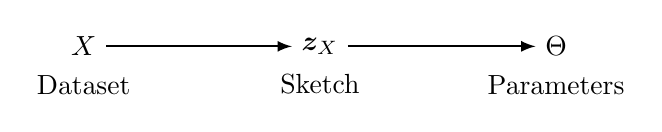
\begin{tikzpicture}
	% Place nodes
	\node [label=below:Dataset] (dataset) at (0,0) {$X$};
	\node [label=below:Sketch] (sketch) at (3,0) {$\Vec{z}_X$};
	\node [label=below:Parameters] (parameters) at (6,0) {$\Theta$};
	
	% Draw edges
	\draw [->, thick, -latex] (dataset) -- (sketch);
	\draw [->, thick, -latex] (sketch) -- (parameters);
	\end{tikzpicture}
	\caption{Compressive learning .}
	\label{fig:CL}
	\end {figure}


\begin{equation}
\label{eq:sketching}
	\Vec{z}_X := \frac{1}{n} \sum_{i = 1}^n \Phi(\Vec{x}_i)
\end{equation}

See \cite{gribonval2017compressive} for a complete introduction to compressive learning.

\section{An overview of Pycle}
% TODO explain how it is structured, how to use


\subsection{Requirements}
The Pycle package builds on a set of standard Python libraries, that are required to run it: % standard in scientific computing with python
\begin{itemize}
	\item \code{numpy}
	\item \code{scipy}
	\item \code{matplotlib}
\end{itemize}

% You can install those packages by...

\subsection{Typical workflow}

A typical use of Pycle follows the following steps:
\begin{enumerate}
	\item Design a sketch operator, then sketch the dataset using the \code{sketching.py} module.
	\item Extract a model from the sketch by a compressive learning method contained in the \code{compressive\_learning.py} module.
\end{enumerate}




	
		
\begin{figure}[!htb]
	\centering
		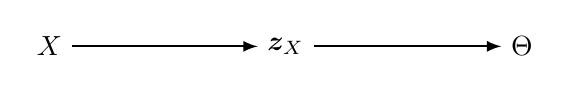
\begin{tikzpicture}
		% Place nodes
		\node (dataset) at (0,0) {$X$};
		\node (sketch) at (3,0) {$\Vec{z}_X$};
		\node (parameters) at (6,0) {$\Theta$};
		
		% Draw edges
		\draw [->, thick, -latex] (dataset) -- (sketch);
		\draw [->, thick, -latex] (sketch) -- (parameters);
		\end{tikzpicture}
	\caption{Flowchart of a typical compressive learning execution with Pycle.}
	\label{fig:flowchart}
\end {figure}
		



\section{A tutorial tour of \code{pycle}}
We now explain the core features of \code{pycle}. I'll go over each of the submodules one by one and introduce, in a ``tutorial style'', the most important tools they provide. Our focus being on understanding, this section is neither concise nor exhaustive (however, section \ref{sec:documentation} is a methodical list of all the toolbox features).
\subsection{Sketching} 
To use the \code{sketching} submodule, you first need to import it (to spare me some typing, I personally like tu use \code{sk} as shorthand). Usual sketching as defined in~\eqref{eq:sketching} can then be done by calling \code{sk.computeSketch} as follows.
\begin{lstlisting}
import pycle.sketching as sk

X = ...    # load a numpy array of dimension (n,d)
Phi = ... # sketch feature map, see later

z = sk.computeSketch(X,Phi)
\end{lstlisting}

\noindent As you might have guessed, \code{sk.computeSketch(dataset,featureMap)} requires two arguments: the dataset $X$, and the feature map $\Phi$. Let's start with the simplest one: the dataset $X$ should be given as a 2d numpy array of dimensions $(n,d)$.

\note{\textbf{Matrix representation conventions}.
We follow the same convention as most mainstream Python ML modules: the dataset, that we mathematically describe as $X = (\Vec{x}_i \in \mathbb R^d)_{i = 1}^n \in \mathbb R^{d \times n}$, is represented by a numpy array of shape $(n,d)$. In particular, \code{X[0]} references $\Vec{x_1}$: note the awkward inversion of dimension order. For matrices that don't represent datasets (e.g., $\Omega$ in the examples below), we stick to the mathematical convention instead, i.e., a matrix of the type $\mathbb R^{a \times b}$ is represented by a numpy array of shape $(a,b)$.}

\noindent The feature map argument can be specified in one of the two following ways. Either---and this is the method I recommend---you give an instance of a \code{FeatureMap} object (explained below), or you directly provide a callable Python function (e.g., to compute the second-order moments for the sketch, write \code{Phi = lambda x: x**2}). Note that the second method is proposed for research purposes, in the case you want to construct a custom feature map that cannot be instantiated with the methods provided within the \code{FeatureMap} class.

% I arrived here

\note{\textbf{FeatureMap objects}.
Why do we use \code{FeatureMap} objects instead of (Python) functions to represent... well, (mathematical) functions? Because we often require additional metadata/methods about $\Phi$ (e.g., target dimension $m$, jacobian $\nabla\Phi$,...). All these parameters and methods are conveniently packaged inside \code{FeatureMap} objects.}

\emph{Voil�}, you know the basics of how the \code{sketching} submodule is used! Well, OK, all we saw was a function that computes an average, but hey, that's like, the essence of sketching, it's not my fault. Luckily for you, \code{sketching} has much more to offer. First and foremost, I'll demonstrate the whole zoo of feature maps that are readily available---I promise you, you'll construct your \code{FeatureMap} object $\Phi$ in no more than two lines of code. After this comes more advanced methods of the toolbox that you may not need right away: I'll show how to automatically select the \emph{scale hyper-parameter} in the aforementioned feature maps (which in practice can be hard to guess \emph{a priori}); I'll then finally explain \code{pycle}s functions for sketching with Differential Privacy guarantees. 

\subsubsection{Painless instantiation of standard feature maps: the \code{SimpleFeatureMap} class}
All feature maps used in CL up to now are of the following form, which we call ``Simple Feature Map'',
\begin{equation}
\Phi(\Vec{x}) = f(\Omega^T\Vec{x} + \Vec{\xi}), \quad \text{where} \quad \Omega = [\Vec{\omega}_1, \cdots, \Vec{\omega}_m] \in \mathbb{R}^{d \times m}, \: \Vec{\xi} = [\xi_1, \cdots, \xi_m]^T \in \mathbb{R}^{m},
\end{equation}
and $f$ is a point-wise nonlinearity (i.e., $\Phi_j(\Vec{x}) = f(\Vec{\omega}_j^T\Vec{x} + \xi_j)$ for all $j$). In general, you can instantiate such a nonlinearity in pycle in the following way:
\begin{lstlisting}
import pycle.sketching as sk

f = ...       # nonlinearity (Python function, tuple or string)
Omega = ...   # (d,m) numpy array
xi = ...      # (m,) numpy array
Phi = sk.SimpleFeatureMap(f, Omega, xi)
\end{lstlisting}

Moreover, the ``usual'' arguments for this simple feature map can be easily called, as we explain below.
\begin{itemize}
	\item nonlinearity
	\item projection
	\item dithering
\end{itemize}

\subsubsection{Designing the sampling pattern in the feature maps: the \code{estimateSigma} function}

\subsubsection{Guaranteeing the Differential Privacy of sketching: the \code{computeSketch\_DP} function}


% Explain the FeatureMap

% Come back to the code

% Privacy

\subsection{Learning} 

\subsection{Utilities} 


\section{Documentation}
\label{sec:documentation}
\subsection{Sketching methods} 

\subsection{Learning tools} 

\subsection{Utilities} 




\section{Conclusion: going further}
My primary goals for \code{pycle} are that it should be:
\begin{itemize}
	\item \textbf{intuitive to use:} practitioners with no background knowledge in compressive learning and little experience in Python should be able to use it to implement compressive learning in their own projects;
	\item \textbf{flexible to new features:} researchers with interest in compressive learning (that want to try out new methods/techniques in CL) should be able to easily extend this code to suit their own needs, without having to re-write things from scratch (and eventually, suggesting to add some features to the toolbox);
	\item \textbf{efficient to run:} the main motivation of compressive learning is based on the fact that it can be much more memory- and time-efficient than traditional learning methods, so the performances of the toolbox should fulfill that promise (note: this goal is still a challenge for me, this item is rather wishful thinking). 
\end{itemize}
With this in mind, if you have any suggestions to improve the toolbox, please don't hesitate to contact me!

\newpage
\bibliography{guidebib.bib}
\bibliographystyle{ieeetr}


\end{document}
